% Options for packages loaded elsewhere
\PassOptionsToPackage{unicode}{hyperref}
\PassOptionsToPackage{hyphens}{url}
%
\documentclass[
]{article}
\usepackage{amsmath,amssymb}
\usepackage{lmodern}
\usepackage{iftex}
\ifPDFTeX
  \usepackage[T1]{fontenc}
  \usepackage[utf8]{inputenc}
  \usepackage{textcomp} % provide euro and other symbols
\else % if luatex or xetex
  \usepackage{unicode-math}
  \defaultfontfeatures{Scale=MatchLowercase}
  \defaultfontfeatures[\rmfamily]{Ligatures=TeX,Scale=1}
\fi
% Use upquote if available, for straight quotes in verbatim environments
\IfFileExists{upquote.sty}{\usepackage{upquote}}{}
\IfFileExists{microtype.sty}{% use microtype if available
  \usepackage[]{microtype}
  \UseMicrotypeSet[protrusion]{basicmath} % disable protrusion for tt fonts
}{}
\makeatletter
\@ifundefined{KOMAClassName}{% if non-KOMA class
  \IfFileExists{parskip.sty}{%
    \usepackage{parskip}
  }{% else
    \setlength{\parindent}{0pt}
    \setlength{\parskip}{6pt plus 2pt minus 1pt}}
}{% if KOMA class
  \KOMAoptions{parskip=half}}
\makeatother
\usepackage{xcolor}
\usepackage[margin=1in]{geometry}
\usepackage{color}
\usepackage{fancyvrb}
\newcommand{\VerbBar}{|}
\newcommand{\VERB}{\Verb[commandchars=\\\{\}]}
\DefineVerbatimEnvironment{Highlighting}{Verbatim}{commandchars=\\\{\}}
% Add ',fontsize=\small' for more characters per line
\usepackage{framed}
\definecolor{shadecolor}{RGB}{248,248,248}
\newenvironment{Shaded}{\begin{snugshade}}{\end{snugshade}}
\newcommand{\AlertTok}[1]{\textcolor[rgb]{0.94,0.16,0.16}{#1}}
\newcommand{\AnnotationTok}[1]{\textcolor[rgb]{0.56,0.35,0.01}{\textbf{\textit{#1}}}}
\newcommand{\AttributeTok}[1]{\textcolor[rgb]{0.77,0.63,0.00}{#1}}
\newcommand{\BaseNTok}[1]{\textcolor[rgb]{0.00,0.00,0.81}{#1}}
\newcommand{\BuiltInTok}[1]{#1}
\newcommand{\CharTok}[1]{\textcolor[rgb]{0.31,0.60,0.02}{#1}}
\newcommand{\CommentTok}[1]{\textcolor[rgb]{0.56,0.35,0.01}{\textit{#1}}}
\newcommand{\CommentVarTok}[1]{\textcolor[rgb]{0.56,0.35,0.01}{\textbf{\textit{#1}}}}
\newcommand{\ConstantTok}[1]{\textcolor[rgb]{0.00,0.00,0.00}{#1}}
\newcommand{\ControlFlowTok}[1]{\textcolor[rgb]{0.13,0.29,0.53}{\textbf{#1}}}
\newcommand{\DataTypeTok}[1]{\textcolor[rgb]{0.13,0.29,0.53}{#1}}
\newcommand{\DecValTok}[1]{\textcolor[rgb]{0.00,0.00,0.81}{#1}}
\newcommand{\DocumentationTok}[1]{\textcolor[rgb]{0.56,0.35,0.01}{\textbf{\textit{#1}}}}
\newcommand{\ErrorTok}[1]{\textcolor[rgb]{0.64,0.00,0.00}{\textbf{#1}}}
\newcommand{\ExtensionTok}[1]{#1}
\newcommand{\FloatTok}[1]{\textcolor[rgb]{0.00,0.00,0.81}{#1}}
\newcommand{\FunctionTok}[1]{\textcolor[rgb]{0.00,0.00,0.00}{#1}}
\newcommand{\ImportTok}[1]{#1}
\newcommand{\InformationTok}[1]{\textcolor[rgb]{0.56,0.35,0.01}{\textbf{\textit{#1}}}}
\newcommand{\KeywordTok}[1]{\textcolor[rgb]{0.13,0.29,0.53}{\textbf{#1}}}
\newcommand{\NormalTok}[1]{#1}
\newcommand{\OperatorTok}[1]{\textcolor[rgb]{0.81,0.36,0.00}{\textbf{#1}}}
\newcommand{\OtherTok}[1]{\textcolor[rgb]{0.56,0.35,0.01}{#1}}
\newcommand{\PreprocessorTok}[1]{\textcolor[rgb]{0.56,0.35,0.01}{\textit{#1}}}
\newcommand{\RegionMarkerTok}[1]{#1}
\newcommand{\SpecialCharTok}[1]{\textcolor[rgb]{0.00,0.00,0.00}{#1}}
\newcommand{\SpecialStringTok}[1]{\textcolor[rgb]{0.31,0.60,0.02}{#1}}
\newcommand{\StringTok}[1]{\textcolor[rgb]{0.31,0.60,0.02}{#1}}
\newcommand{\VariableTok}[1]{\textcolor[rgb]{0.00,0.00,0.00}{#1}}
\newcommand{\VerbatimStringTok}[1]{\textcolor[rgb]{0.31,0.60,0.02}{#1}}
\newcommand{\WarningTok}[1]{\textcolor[rgb]{0.56,0.35,0.01}{\textbf{\textit{#1}}}}
\usepackage{longtable,booktabs,array}
\usepackage{calc} % for calculating minipage widths
% Correct order of tables after \paragraph or \subparagraph
\usepackage{etoolbox}
\makeatletter
\patchcmd\longtable{\par}{\if@noskipsec\mbox{}\fi\par}{}{}
\makeatother
% Allow footnotes in longtable head/foot
\IfFileExists{footnotehyper.sty}{\usepackage{footnotehyper}}{\usepackage{footnote}}
\makesavenoteenv{longtable}
\usepackage{graphicx}
\makeatletter
\def\maxwidth{\ifdim\Gin@nat@width>\linewidth\linewidth\else\Gin@nat@width\fi}
\def\maxheight{\ifdim\Gin@nat@height>\textheight\textheight\else\Gin@nat@height\fi}
\makeatother
% Scale images if necessary, so that they will not overflow the page
% margins by default, and it is still possible to overwrite the defaults
% using explicit options in \includegraphics[width, height, ...]{}
\setkeys{Gin}{width=\maxwidth,height=\maxheight,keepaspectratio}
% Set default figure placement to htbp
\makeatletter
\def\fps@figure{htbp}
\makeatother
\setlength{\emergencystretch}{3em} % prevent overfull lines
\providecommand{\tightlist}{%
  \setlength{\itemsep}{0pt}\setlength{\parskip}{0pt}}
\setcounter{secnumdepth}{-\maxdimen} % remove section numbering
\usepackage{booktabs}
\usepackage{longtable}
\usepackage{array}
\usepackage{multirow}
\usepackage{wrapfig}
\usepackage{float}
\usepackage{colortbl}
\usepackage{pdflscape}
\usepackage{tabu}
\usepackage{threeparttable}
\usepackage{threeparttablex}
\usepackage[normalem]{ulem}
\usepackage{makecell}
\usepackage{xcolor}
\ifLuaTeX
  \usepackage{selnolig}  % disable illegal ligatures
\fi
\IfFileExists{bookmark.sty}{\usepackage{bookmark}}{\usepackage{hyperref}}
\IfFileExists{xurl.sty}{\usepackage{xurl}}{} % add URL line breaks if available
\urlstyle{same} % disable monospaced font for URLs
\hypersetup{
  pdftitle={Network Analysis and Centrality Measures},
  hidelinks,
  pdfcreator={LaTeX via pandoc}}

\title{Network Analysis and Centrality Measures}
\author{}
\date{\vspace{-2.5em}}

\begin{document}
\maketitle

\begin{Shaded}
\begin{Highlighting}[]
\NormalTok{knitr}\SpecialCharTok{::}\NormalTok{opts\_chunk}\SpecialCharTok{$}\FunctionTok{set}\NormalTok{(}\AttributeTok{echo =} \ConstantTok{TRUE}\NormalTok{)}
\FunctionTok{library}\NormalTok{(tidyverse)}
\end{Highlighting}
\end{Shaded}

\begin{verbatim}
## Warning: package 'ggplot2' was built under R version 4.3.1
\end{verbatim}

\begin{verbatim}
## Warning: package 'lubridate' was built under R version 4.3.1
\end{verbatim}

\begin{verbatim}
## -- Attaching core tidyverse packages ------------------------ tidyverse 2.0.0 --
## v dplyr     1.1.2     v readr     2.1.4
## v forcats   1.0.0     v stringr   1.5.0
## v ggplot2   3.5.0     v tibble    3.2.1
## v lubridate 1.9.3     v tidyr     1.3.0
## v purrr     1.0.1     
## -- Conflicts ------------------------------------------ tidyverse_conflicts() --
## x dplyr::filter() masks stats::filter()
## x dplyr::lag()    masks stats::lag()
## i Use the conflicted package (<http://conflicted.r-lib.org/>) to force all conflicts to become errors
\end{verbatim}

\begin{Shaded}
\begin{Highlighting}[]
\FunctionTok{library}\NormalTok{(igraph)}
\end{Highlighting}
\end{Shaded}

\begin{verbatim}
## Warning: package 'igraph' was built under R version 4.3.1
\end{verbatim}

\begin{verbatim}
## 
## Attaching package: 'igraph'
## 
## The following objects are masked from 'package:lubridate':
## 
##     %--%, union
## 
## The following objects are masked from 'package:dplyr':
## 
##     as_data_frame, groups, union
## 
## The following objects are masked from 'package:purrr':
## 
##     compose, simplify
## 
## The following object is masked from 'package:tidyr':
## 
##     crossing
## 
## The following object is masked from 'package:tibble':
## 
##     as_data_frame
## 
## The following objects are masked from 'package:stats':
## 
##     decompose, spectrum
## 
## The following object is masked from 'package:base':
## 
##     union
\end{verbatim}

\begin{Shaded}
\begin{Highlighting}[]
\FunctionTok{library}\NormalTok{(kableExtra)}
\end{Highlighting}
\end{Shaded}

\begin{verbatim}
## Warning: package 'kableExtra' was built under R version 4.3.1
\end{verbatim}

\begin{verbatim}
## 
## Attaching package: 'kableExtra'
## 
## The following object is masked from 'package:dplyr':
## 
##     group_rows
\end{verbatim}

\begin{Shaded}
\begin{Highlighting}[]
\CommentTok{\# Create a blank matrix}
\NormalTok{adjacency\_matrix }\OtherTok{\textless{}{-}} \FunctionTok{matrix}\NormalTok{(}\DecValTok{0}\NormalTok{, }\AttributeTok{nrow=}\DecValTok{10}\NormalTok{, }\AttributeTok{ncol=}\DecValTok{10}\NormalTok{)}

\CommentTok{\# Define the names for the rows and columns for clarity}
\FunctionTok{rownames}\NormalTok{(adjacency\_matrix) }\OtherTok{\textless{}{-}} \FunctionTok{c}\NormalTok{(}\StringTok{"5"}\NormalTok{, }\StringTok{"6"}\NormalTok{, }\StringTok{"D"}\NormalTok{, }\StringTok{"3"}\NormalTok{, }\StringTok{"4"}\NormalTok{, }\StringTok{"B"}\NormalTok{, }\StringTok{"C"}\NormalTok{, }\StringTok{"A"}\NormalTok{, }\StringTok{"2"}\NormalTok{, }\StringTok{"1"}\NormalTok{)}
\FunctionTok{colnames}\NormalTok{(adjacency\_matrix) }\OtherTok{\textless{}{-}} \FunctionTok{c}\NormalTok{(}\StringTok{"5"}\NormalTok{, }\StringTok{"6"}\NormalTok{, }\StringTok{"D"}\NormalTok{, }\StringTok{"3"}\NormalTok{, }\StringTok{"4"}\NormalTok{, }\StringTok{"B"}\NormalTok{, }\StringTok{"C"}\NormalTok{, }\StringTok{"A"}\NormalTok{, }\StringTok{"2"}\NormalTok{, }\StringTok{"1"}\NormalTok{)}

\CommentTok{\# Connections for 5}
\NormalTok{adjacency\_matrix[}\StringTok{"5"}\NormalTok{, }\FunctionTok{c}\NormalTok{(}\StringTok{"D"}\NormalTok{, }\StringTok{"6"}\NormalTok{, }\StringTok{"3"}\NormalTok{)] }\OtherTok{\textless{}{-}} \DecValTok{1}

\CommentTok{\# Connections for 6}
\NormalTok{adjacency\_matrix[}\StringTok{"6"}\NormalTok{, }\FunctionTok{c}\NormalTok{(}\StringTok{"D"}\NormalTok{, }\StringTok{"B"}\NormalTok{, }\StringTok{"5"}\NormalTok{)] }\OtherTok{\textless{}{-}} \DecValTok{1}

\CommentTok{\# Connections for D}
\NormalTok{adjacency\_matrix[}\StringTok{"D"}\NormalTok{, }\FunctionTok{c}\NormalTok{(}\StringTok{"5"}\NormalTok{, }\StringTok{"6"}\NormalTok{, }\StringTok{"3"}\NormalTok{, }\StringTok{"B"}\NormalTok{, }\StringTok{"C"}\NormalTok{)] }\OtherTok{\textless{}{-}} \DecValTok{1}

\CommentTok{\# Connections for 3}
\NormalTok{adjacency\_matrix[}\StringTok{"3"}\NormalTok{, }\FunctionTok{c}\NormalTok{(}\StringTok{"D"}\NormalTok{, }\StringTok{"4"}\NormalTok{, }\StringTok{"C"}\NormalTok{, }\StringTok{"B"}\NormalTok{, }\StringTok{"5"}\NormalTok{)] }\OtherTok{\textless{}{-}} \DecValTok{1}

\CommentTok{\# Connections for 4}
\NormalTok{adjacency\_matrix[}\StringTok{"4"}\NormalTok{, }\FunctionTok{c}\NormalTok{(}\StringTok{"3"}\NormalTok{, }\StringTok{"C"}\NormalTok{)] }\OtherTok{\textless{}{-}} \DecValTok{1}

\CommentTok{\# Connections for B}
\NormalTok{adjacency\_matrix[}\StringTok{"B"}\NormalTok{, }\FunctionTok{c}\NormalTok{(}\StringTok{"6"}\NormalTok{, }\StringTok{"D"}\NormalTok{, }\StringTok{"C"}\NormalTok{, }\StringTok{"A"}\NormalTok{, }\StringTok{"3"}\NormalTok{)] }\OtherTok{\textless{}{-}} \DecValTok{1}

\CommentTok{\# Connections for C}
\NormalTok{adjacency\_matrix[}\StringTok{"C"}\NormalTok{, }\FunctionTok{c}\NormalTok{(}\StringTok{"3"}\NormalTok{, }\StringTok{"4"}\NormalTok{, }\StringTok{"B"}\NormalTok{, }\StringTok{"D"}\NormalTok{, }\StringTok{"A"}\NormalTok{)] }\OtherTok{\textless{}{-}} \DecValTok{1}

\CommentTok{\# Connections for A}
\NormalTok{adjacency\_matrix[}\StringTok{"A"}\NormalTok{, }\FunctionTok{c}\NormalTok{(}\StringTok{"C"}\NormalTok{, }\StringTok{"B"}\NormalTok{, }\StringTok{"2"}\NormalTok{)] }\OtherTok{\textless{}{-}} \DecValTok{1}

\CommentTok{\# Connections for 2}
\NormalTok{adjacency\_matrix[}\StringTok{"2"}\NormalTok{, }\FunctionTok{c}\NormalTok{(}\StringTok{"A"}\NormalTok{, }\StringTok{"1"}\NormalTok{)] }\OtherTok{\textless{}{-}} \DecValTok{1}

\CommentTok{\# Connections for 1}
\NormalTok{adjacency\_matrix[}\StringTok{"1"}\NormalTok{, }\StringTok{"2"}\NormalTok{] }\OtherTok{\textless{}{-}} \DecValTok{1}

\CommentTok{\# Since the graph is undirected, we mirror the matrix along the diagonal}
\NormalTok{adjacency\_matrix }\OtherTok{\textless{}{-}}\NormalTok{ adjacency\_matrix }\SpecialCharTok{+} \FunctionTok{t}\NormalTok{(adjacency\_matrix)}
\CommentTok{\# convert where the value is 2 to 1}
\NormalTok{adjacency\_matrix[adjacency\_matrix }\SpecialCharTok{==} \DecValTok{2}\NormalTok{] }\OtherTok{\textless{}{-}} \DecValTok{1}

\CommentTok{\#sort the matrix}
\NormalTok{adjacency\_matrix }\OtherTok{\textless{}{-}}\NormalTok{ adjacency\_matrix[}\FunctionTok{order}\NormalTok{(}\FunctionTok{rownames}\NormalTok{(adjacency\_matrix)), }\FunctionTok{order}\NormalTok{(}\FunctionTok{colnames}\NormalTok{(adjacency\_matrix))]}

\CommentTok{\# Print out the matrix}
\NormalTok{adjacency\_matrix}
\end{Highlighting}
\end{Shaded}

\begin{verbatim}
##   1 2 3 4 5 6 A B C D
## 1 0 1 0 0 0 0 0 0 0 0
## 2 1 0 0 0 0 0 1 0 0 0
## 3 0 0 0 1 1 0 0 1 1 1
## 4 0 0 1 0 0 0 0 0 1 0
## 5 0 0 1 0 0 1 0 0 0 1
## 6 0 0 0 0 1 0 0 1 0 1
## A 0 1 0 0 0 0 0 1 1 0
## B 0 0 1 0 0 1 1 0 1 1
## C 0 0 1 1 0 0 1 1 0 1
## D 0 0 1 0 1 1 0 1 1 0
\end{verbatim}

\begin{Shaded}
\begin{Highlighting}[]
\FunctionTok{library}\NormalTok{(igraph)}

\NormalTok{graph }\OtherTok{\textless{}{-}} \FunctionTok{graph\_from\_adjacency\_matrix}\NormalTok{(adjacency\_matrix, }\AttributeTok{mode =} \StringTok{"undirected"}\NormalTok{)}

\CommentTok{\# Plot the graph}
\FunctionTok{plot}\NormalTok{(graph, }\AttributeTok{layout =} \FunctionTok{layout\_nicely}\NormalTok{(graph), }\AttributeTok{vertex.color =} \StringTok{"skyblue"}\NormalTok{, }\AttributeTok{edge.arrow.size =} \FloatTok{0.5}\NormalTok{)}
\end{Highlighting}
\end{Shaded}

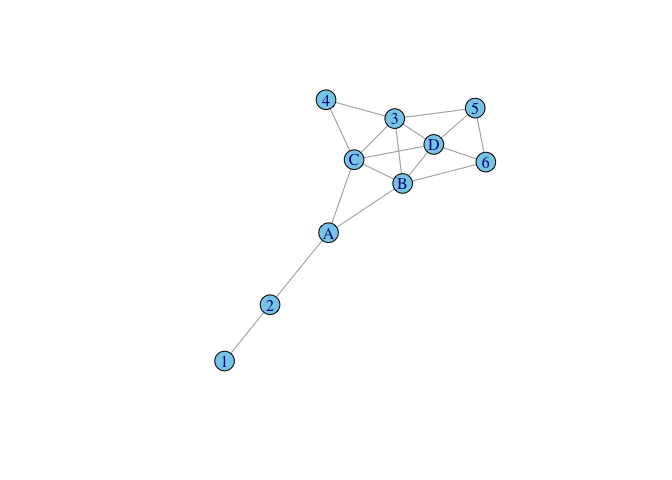
\includegraphics{/Users/kaz/DataspellProjects/Org-Analytics/Ex2/ex2_files/figure-latex/unnamed-chunk-2-1.pdf}

\begin{Shaded}
\begin{Highlighting}[]
\CommentTok{\# Calculate degree centrality for all nodes}
\NormalTok{degree\_centrality }\OtherTok{\textless{}{-}} \FunctionTok{degree}\NormalTok{(graph, }\AttributeTok{mode =} \StringTok{"all"}\NormalTok{)}

\CommentTok{\# Calculate closeness centrality for all nodes}
\NormalTok{closeness\_centrality }\OtherTok{\textless{}{-}} \FunctionTok{closeness}\NormalTok{(graph, }\AttributeTok{mode =} \StringTok{"all"}\NormalTok{)}

\CommentTok{\# Calculate betweenness centrality for all nodes}
\NormalTok{betweenness\_centrality }\OtherTok{\textless{}{-}} \FunctionTok{betweenness}\NormalTok{(graph, }\AttributeTok{directed =} \ConstantTok{FALSE}\NormalTok{, }\AttributeTok{normalized =} \ConstantTok{TRUE}\NormalTok{)}

\NormalTok{centrality\_measures\_all }\OtherTok{\textless{}{-}} \FunctionTok{data.frame}\NormalTok{(}
  \AttributeTok{Degree =}\NormalTok{ degree\_centrality,}
  \AttributeTok{Closeness =}\NormalTok{ closeness\_centrality,}
  \AttributeTok{Betweenness =}\NormalTok{ betweenness\_centrality}
\NormalTok{)}

\NormalTok{centrality\_measures\_all}
\end{Highlighting}
\end{Shaded}

\begin{verbatim}
##   Degree  Closeness Betweenness
## 1      1 0.03333333  0.00000000
## 2      2 0.04545455  0.22222222
## 3      5 0.06250000  0.12870370
## 4      2 0.05000000  0.00000000
## 5      3 0.04761905  0.01481481
## 6      3 0.05263158  0.02592593
## A      3 0.06250000  0.38888889
## B      5 0.07142857  0.25092593
## C      5 0.07142857  0.23888889
## D      5 0.06250000  0.09074074
\end{verbatim}

\begin{Shaded}
\begin{Highlighting}[]
\CommentTok{\# Extract the centralities for seats A{-}D}
\NormalTok{seat\_choices }\OtherTok{\textless{}{-}} \FunctionTok{c}\NormalTok{(}\StringTok{\textquotesingle{}A\textquotesingle{}}\NormalTok{, }\StringTok{\textquotesingle{}B\textquotesingle{}}\NormalTok{, }\StringTok{\textquotesingle{}C\textquotesingle{}}\NormalTok{, }\StringTok{\textquotesingle{}D\textquotesingle{}}\NormalTok{)}
\NormalTok{centrality\_measures }\OtherTok{\textless{}{-}} \FunctionTok{data.frame}\NormalTok{(}
  \AttributeTok{Degree =}\NormalTok{ degree\_centrality[seat\_choices],}
  \AttributeTok{Closeness =}\NormalTok{ closeness\_centrality[seat\_choices],}
  \AttributeTok{Betweenness =}\NormalTok{ betweenness\_centrality[seat\_choices]}
\NormalTok{)}
\FunctionTok{rownames}\NormalTok{(centrality\_measures) }\OtherTok{\textless{}{-}}\NormalTok{ seat\_choices}
\end{Highlighting}
\end{Shaded}

Centrality Measures for Seats A-D

\begin{longtable}[]{@{}lrrr@{}}
\toprule()
& Degree & Closeness & Betweenness \\
\midrule()
\endhead
A & 3 & 0.06250 & 0.388889 \\
B & 5 & 0.07143 & 0.250926 \\
C & 5 & 0.07143 & 0.238889 \\
D & 5 & 0.06250 & 0.090741 \\
\bottomrule()
\end{longtable}

\hypertarget{seat-a}{%
\subsubsection{Seat A}\label{seat-a}}

\begin{itemize}
\tightlist
\item
  \textbf{Key Feature}: Highest betweenness centrality, lowest degree
  centrality.
\item
  \textbf{Benefit}: Sitting in Seat A positions you as a key bridge in
  the network, connecting different coworker groups. This is beneficial
  for meeting diverse individuals --\textgreater{} can offer broad
  insights into the company culture and cross-departmental projects.
\item
  \textbf{Drawback}: The lower degree centrality means you might have
  fewer direct connections, potentially making it harder to quickly form
  a close-knit group of friends.
\end{itemize}

\hypertarget{seat-b}{%
\subsubsection{Seat B}\label{seat-b}}

\begin{itemize}
\tightlist
\item
  \textbf{Key Feature}: High degree and closeness centrality.
\item
  \textbf{Benefit}: access to a larger direct network and easier
  communication with others due to the high closeness centrality,
  facilitating exchange of information and support.
\item
  \textbf{Drawback}: the focus here is less on being the sole connector
  and more on being part of a cohesive network, which might
  \textbf{limit exclusive networking}.
\end{itemize}

\hypertarget{seat-c}{%
\subsubsection{Seat C}\label{seat-c}}

\begin{itemize}
\tightlist
\item
  \textbf{Key Feature}: Similar to Seat B.
\end{itemize}

\hypertarget{seat-d}{%
\subsubsection{Seat D}\label{seat-d}}

\begin{itemize}
\tightlist
\item
  \textbf{Key Feature}: High degree and closeness centrality but lowest
  betweenness centrality.
\item
  \textbf{Benefit}: Similar to B and C
\item
  \textbf{Drawback}: The lowest betweenness centrality = less ideal for
  those looking to play a bridging role between unconnected coworker
  groups (less networkhub role).
\end{itemize}

\textbf{In Summary}: - \textbf{For broad networking across diverse
groups}: \textbf{Seat A} - \textbf{For quickly establishing a strong,
central presence in your immediate network}: \textbf{Seats B, C, and D}

\textbf{What if\ldots{}} - if you want to make the strongest bond with
one person in the bus, where should you sit, assuming every seat is
available? - 1 or 2 - they have the least number of connections, they
are far from the rest of the network, and they are not in the middle of
the network.

\begin{quote}
If you choose 1, then 2 is your only bet and 2 has more
``opportunities''. So if you want to make the strongest connection, you
would sit in seat 2 and only talk to the person in seat 1.
\end{quote}

\begin{Shaded}
\begin{Highlighting}[]
\NormalTok{degree\_centrality }\OtherTok{\textless{}{-}} \FunctionTok{degree}\NormalTok{(graph, }\AttributeTok{mode =} \StringTok{"all"}\NormalTok{)}
\NormalTok{closeness\_centrality }\OtherTok{\textless{}{-}} \FunctionTok{closeness}\NormalTok{(graph, }\AttributeTok{mode =} \StringTok{"all"}\NormalTok{)}
\NormalTok{betweenness\_centrality }\OtherTok{\textless{}{-}} \FunctionTok{betweenness}\NormalTok{(graph, }\AttributeTok{directed =} \ConstantTok{FALSE}\NormalTok{)}

\CommentTok{\# Set up the layout of the graph just once to use in all plots}
\NormalTok{layout }\OtherTok{\textless{}{-}} \FunctionTok{layout\_with\_fr}\NormalTok{(graph)}

\CommentTok{\# Set up the plotting area}
\FunctionTok{par}\NormalTok{(}\AttributeTok{mfrow =} \FunctionTok{c}\NormalTok{(}\DecValTok{2}\NormalTok{, }\DecValTok{2}\NormalTok{))}

\CommentTok{\# Degree Centrality Plot}
\FunctionTok{plot}\NormalTok{(graph, }\AttributeTok{layout =}\NormalTok{ layout,}
     \AttributeTok{vertex.label =} \FunctionTok{V}\NormalTok{(graph)}\SpecialCharTok{$}\NormalTok{name,}
     \AttributeTok{vertex.size =}\NormalTok{ degree\_centrality }\SpecialCharTok{*} \DecValTok{5}\NormalTok{,}
     \AttributeTok{vertex.label.cex =} \FloatTok{0.8}\NormalTok{,}
     \AttributeTok{edge.arrow.size =} \FloatTok{0.5}\NormalTok{,}
     \AttributeTok{main =} \StringTok{"Degree Centrality"}\NormalTok{)}

\CommentTok{\# Closeness Centrality Plot}
\FunctionTok{plot}\NormalTok{(graph, }\AttributeTok{layout =}\NormalTok{ layout,}
     \AttributeTok{vertex.label =} \FunctionTok{V}\NormalTok{(graph)}\SpecialCharTok{$}\NormalTok{name,}
     \AttributeTok{vertex.size =}\NormalTok{ closeness\_centrality }\SpecialCharTok{*} \DecValTok{500}\NormalTok{,  }\CommentTok{\# Scale factor to make the sizes visible, adjust as needed}
     \AttributeTok{vertex.label.cex =} \FloatTok{0.8}\NormalTok{,}
     \AttributeTok{edge.arrow.size =} \FloatTok{0.5}\NormalTok{,}
     \AttributeTok{main =} \StringTok{"Closeness Centrality"}\NormalTok{)}

\CommentTok{\# Betweenness Centrality Plot}
\FunctionTok{plot}\NormalTok{(graph, }\AttributeTok{layout =}\NormalTok{ layout,}
     \AttributeTok{vertex.label =} \FunctionTok{V}\NormalTok{(graph)}\SpecialCharTok{$}\NormalTok{name,}
     \AttributeTok{vertex.size =}\NormalTok{ betweenness\_centrality }\SpecialCharTok{/} \FunctionTok{max}\NormalTok{(betweenness\_centrality) }\SpecialCharTok{*} \DecValTok{50}\NormalTok{,  }\CommentTok{\# Normalize and scale, adjust as needed}
     \AttributeTok{vertex.label.cex =} \FloatTok{0.8}\NormalTok{,}
     \AttributeTok{edge.arrow.size =} \FloatTok{0.5}\NormalTok{,}
     \AttributeTok{main =} \StringTok{"Betweenness Centrality"}\NormalTok{)}

\CommentTok{\# Resetting to default single plotting layout}
\FunctionTok{par}\NormalTok{(}\AttributeTok{mfrow =} \FunctionTok{c}\NormalTok{(}\DecValTok{1}\NormalTok{, }\DecValTok{1}\NormalTok{))}
\end{Highlighting}
\end{Shaded}

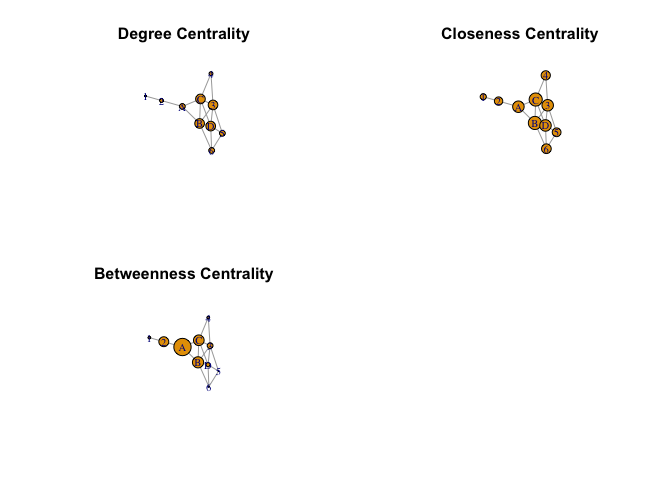
\includegraphics{/Users/kaz/DataspellProjects/Org-Analytics/Ex2/ex2_files/figure-latex/unnamed-chunk-5-1.pdf}

\begin{Shaded}
\begin{Highlighting}[]
\FunctionTok{par}\NormalTok{(}\AttributeTok{mai =} \FunctionTok{c}\NormalTok{(}\DecValTok{0}\NormalTok{, }\DecValTok{0}\NormalTok{, }\FloatTok{0.5}\NormalTok{, }\FloatTok{0.5}\NormalTok{))}
\end{Highlighting}
\end{Shaded}


\end{document}
